\documentclass{beamer}
\usepackage[brazil]{babel}
\usetheme{Madrid}
\usepackage{verbatim}
\usepackage{lmodern}
\usepackage{multirow}
\usepackage{tikz}


% Dados do autor
\author{Heder Dorneles Soares}
\title{Desenvolvimento Web 1}
\institute{IFSP}
\date{\today}

\begin{document}

% Slide de título
\begin{frame}
  \titlepage
\end{frame}



% Slides seguintes...
\begin{frame}
  \frametitle{Introdução}
  HTML é a sigla para \textit{HyperText Markup Language}, que, em português significa linguagem para marcação de hipertexto.
\end{frame}

% Slide de introdução ao HTML
\begin{frame}
  \frametitle{O que é HTML?}
  HTML (\textit{HyperText Markup Language}) é a linguagem de marcação padrão para criar páginas da web. É a base fundamental para construir qualquer site e permite que você defina a estrutura e o conteúdo do documento, como texto, imagens, links, formulários, etc.
\end{frame}

% Slide sobre Tags e Elementos
\begin{frame}
  \frametitle{Tags e Elementos}
  As páginas HTML são construídas usando tags, que são usadas para marcar elementos na página. Cada tag HTML começa com um sinal de menor que ("\(<\)") e termina com um sinal de maior que ("\(>\)"). Um elemento é formado por uma tag de abertura e uma tag de fechamento, envolvendo o conteúdo que deseja-se marcar.

  Exemplo de um parágrafo:
  \texttt{<p>Este é um parágrafo.</p>}
\end{frame}

% Slide sobre Estrutura básica do HTML
\begin{frame}[fragile] % Adicione [fragile] para permitir o uso do ambiente verbatim
  \frametitle{Estrutura básica do HTML}
  Uma página HTML básica geralmente possui a seguinte estrutura:

  \begin{verbatim}
  <!DOCTYPE html>
  <html>
    <head>
      <title>Título da Página</title>
    </head>
    <body>
      <!-- Conteúdo da página aqui -->
    </body>
  </html>
  \end{verbatim}

  O elemento \texttt{<html>} é o contêiner principal, contendo \texttt{<head>} e \texttt{<body>}, onde o conteúdo visível é colocado.
\end{frame}

% Slide sobre Cabeçalhos e Parágrafos
\begin{frame}
  \frametitle{Cabeçalhos e Parágrafos}
  Cabeçalhos (\texttt{<h1>} a \texttt{<h6>}) são usados para títulos e subtítulos na página. Exemplo:

  \texttt{<h1>Título Principal</h1>}\\
  \texttt{<h2>Subtítulo</h2>}\\
  \texttt{<h3>Outro Subtítulo</h3>}\\
  \texttt{<!-- ... -->}\\
  \texttt{<h6>Subtítulo Menor</h6>}

  Parágrafos são marcados com a tag \texttt{<p>}:

  \texttt{<p>Este é um parágrafo.</p>}
\end{frame}

\begin{frame}[fragile]
\frametitle{O que é um Elemento HTML?}

Um elemento HTML é definido por uma tag de abertura, algum conteúdo e uma tag de fechamento:
\begin{verbatim}
<tagname> Conteúdo vai aqui... </tagname>
\end{verbatim}

O elemento HTML é tudo desde a tag de abertura até a tag de fechamento:
\begin{verbatim}
<h1>Meu Primeiro Título</h1>
<p>Meu primeiro parágrafo.</p>
\end{verbatim}

\end{frame}


\begin{frame}[fragile]
\frametitle{A Declaração \texttt{<!DOCTYPE>}}
A declaração \texttt{<!DOCTYPE>} representa o tipo de documento e ajuda os navegadores a exibirem corretamente as páginas da web.

Ela deve aparecer apenas uma vez, no topo da página (antes de qualquer tag HTML).

A declaração \texttt{<!DOCTYPE>} não diferencia letras maiúsculas de minúsculas.

A declaração \texttt{<!DOCTYPE>} para HTML5 é:
\begin{verbatim}
<!DOCTYPE html>
\end{verbatim}
\end{frame}



\begin{frame}[fragile]
\frametitle{Links HTML}

Links HTML são definidos com a tag \texttt{<a>}:\\

\begin{block}{Exemplo}
\begin{verbatim}
<a href="https://www.google.com">Este é um link</a>
\end{verbatim}
\end{block}


O destino do link é especificado no atributo \texttt{href}.

Atributos são usados para fornecer informações adicionais sobre elementos HTML.
\end{frame}


\begin{frame}[fragile]
\frametitle{Imagens HTML}

Imagens HTML são definidas com a tag \texttt{<img>}.

O arquivo de origem (src), texto alternativo (alt), largura (width) e altura (height) são fornecidos como atributos:

\begin{block}{HTML}
\begin{verbatim}
<img src="mapa-do-brasil.jpg" alt="Mapa do Brasil" 
width="104" height="142">
\end{verbatim}   
\end{block}

Podemos usar valores em porcentagem nos atributos width e height. Alt é usado para auxiliar serviços de busca e usuário que utilizam leitores de tela.

\end{frame}


\begin{frame}[fragile]
\frametitle{Atributos da Tag \texttt{<body>}}

A tag \texttt{<body>} é usada para definir o corpo de um documento HTML e contém os seguintes atributos:

\begin{itemize}
  \item \texttt{background}: Especifica a imagem de plano de fundo da página.
  \item \texttt{bgcolor}: Define a cor de fundo da página.
  \item \texttt{text}: Define a cor do texto.
  \item \texttt{link}: Define a cor dos links não visitados.
\end{itemize}

\begin{block}{Exemplo}
\begin{verbatim}
<body bgcolor="#f0f0f0" text="#000000" link="#0000ff">
\end{verbatim}    
\end{block}

\end{frame}


\begin{frame}
\frametitle{Padrão de Cores Hexadecimal no HTML}

Em HTML, as cores são representadas usando o padrão de cores hexadecimal. O formato hexadecimal consiste em seis dígitos alfanuméricos que variam de 0 a 9 e de A a F.

Cada par de dígitos representa a intensidade das cores vermelho (R), verde (G) e azul (B) respectivamente. Os valores vão de 00 (sem intensidade) até FF (máxima intensidade).

Por exemplo:
\begin{itemize}
  \item \texttt{\#FF0000} representa vermelho puro.
  \item \texttt{\#00FF00} representa verde puro.
  \item \texttt{\#0000FF} representa azul puro.
  \item \texttt{\#FFFFFF} representa branco.
  \item \texttt{\#000000} representa preto.
\end{itemize}

\end{frame}


\begin{frame}[fragile]
\frametitle{O Atributo \texttt{style} do HTML}

Definir o estilo de um elemento HTML pode ser feito com o atributo \texttt{style}. O atributo \texttt{style} do HTML possui a seguinte sintaxe:
\begin{block}{Exemplo}
\begin{verbatim}
<tagname style="propriedade:valor;">
\end{verbatim}    
\end{block}


A propriedade e o valor são atributos do CSS\footnote{Nós veremos sobre CSS posteriormente nesta disciplina.}.

\end{frame}


\begin{frame}[fragile]
\frametitle{Exemplo de \texttt{background-color}}

Você pode definir a cor de fundo de um elemento HTML usando o atributo \texttt{style} e a propriedade \texttt{background-color}.

\begin{block}{Exemplo:}
\begin{verbatim}
<p style="background-color: #ff0000; color: #ffffff;">
  Este é um parágrafo com fundo vermelho e texto branco.
</p>
\end{verbatim}
\end{block}


Neste exemplo, a cor de fundo é definida como vermelho (\texttt{\#ff0000}) e a cor do texto é definida como branco (\texttt{\#ffffff}).

\end{frame}


\begin{frame}[fragile]
\frametitle{Cor do Texto}

A propriedade CSS \texttt{color} define a cor do texto para um elemento HTML:

\begin{block}{Exemplo}
\begin{verbatim}
<h1 style="color:blue;">Este é um título</h1>
<p style="color:red;">Este é um parágrafo.</p>
\end{verbatim}
\end{block}

Neste exemplo, a cor do texto para o título é definida como azul (\texttt{blue}) e a cor do texto para o parágrafo é definida como vermelho (\texttt{red}).

\end{frame}



\begin{frame}[fragile]
\frametitle{Fonte, Tamanho e Alinhamento}

No CSS, você pode controlar a fonte, o tamanho da fonte e o alinhamento do texto para um elemento HTML:

\begin{itemize}
  \item \texttt{font-family}: Define o tipo de fonte a ser usada (por exemplo: Arial, Verdana, Courier).
  \item \texttt{font-size}: Define o tamanho da fonte (por exemplo: 12px, 16px).
  \item \texttt{text-align}: Define o alinhamento do texto (por exemplo: left, right, center).
\end{itemize}

\begin{block}{Exemplo}
\begin{verbatim}
<p style="font-family: Arial; font-size: 16px; 
text-align: center;">
  Parágrafo com fonte Arial, tamanho 16px e centralizado.
</p>
\end{verbatim}
\end{block}

Neste exemplo, o parágrafo tem fonte Arial, tamanho de fonte de 16 pixels e está centralizado.

\end{frame}


\begin{frame}{Atividade}
\begin{block}{Exercício}
    Fazer uma página mini-currículo.\\
    Contendo: foto, formatação de fonte, e uso de links.
\end{block}
    
\end{frame}

\begin{frame}
\begin{figure}
    \centering
    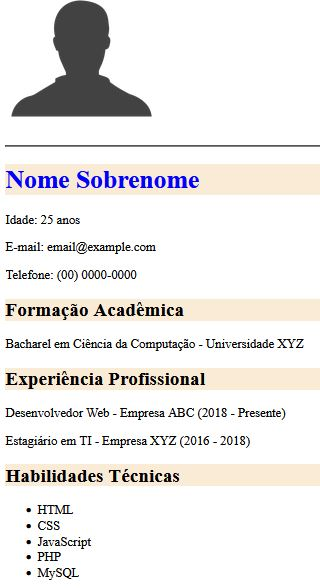
\includegraphics[width=0.4\linewidth]{print-pag.JPG}
    \caption{Mini CV}
    \label{fig:enter-label}
\end{figure}
    
\end{frame}


\begin{frame}[fragile] % Adicione [fragile] para permitir o uso do ambiente verbatim
  \frametitle{Exemplo de Listagem em HTML}
  Suponha que queremos criar uma lista de itens usando HTML:
  \begin{verbatim}
  <ul>
    <li>Item 1</li>
    <li>Item 2</li>
    <li>Item 3</li>
  </ul>
  \end{verbatim}
  Isso será exibido no navegador como:
  \begin{itemize}
    \item Item 1
    \item Item 2
    \item Item 3
  \end{itemize}
\end{frame}

\begin{frame}[fragile] % Adicione [fragile] para permitir o uso do ambiente verbatim
  \frametitle{Exemplo de Listagem Ordenada em HTML}

  Suponha que queremos criar uma lista ordenada de itens usando HTML:

  \begin{verbatim}
  <ol>
    <li>Item 1</li>
    <li>Item 2</li>
    <li>Item 3</li>
  </ol>
  \end{verbatim}

  Isso será exibido no navegador como:

  \begin{enumerate}
    \item Item 1
    \item Item 2
    \item Item 3
  \end{enumerate}
\end{frame}

\begin{frame}[fragile] % Adicione [fragile] para permitir o uso do ambiente verbatim
  \frametitle{Listas de Descrição em HTML}

  HTML também suporta listas de descrição. Uma lista de descrição é uma lista de termos, com uma descrição para cada termo.

  A tag \verb|<dl>| define a lista de descrição, a tag \verb|<dt>| define o termo (nome), e a tag \verb|<dd>| descreve cada termo:

\begin{block}{Exemplo}
\begin{verbatim}
<dl>
  <dt>Portugês</dt>
  <dd>- Aulas às sextas</dd>
  <dt>Matemática</dt>
  <dd>- Aulas às segundas</dd>
</dl>
  \end{verbatim}
\end{block}

\end{frame}


\begin{frame}
  \frametitle{HTML Links - O Atributo \texttt{target}}

  Por padrão, a página vinculada será exibida na janela do navegador atual. Para alterar isso, você deve especificar outro destino para o link.

  O atributo \texttt{target} especifica onde abrir o documento vinculado.

  O atributo \texttt{target} pode ter um dos seguintes valores:

  \begin{description}
    \item[\_self] - Padrão. Abre o documento na mesma janela ou guia em que foi clicado.
    \item[\_blank] - Abre o documento em uma nova janela ou guia.
    \item[\_parent] - Abre o documento no quadro pai.
    \item[\_top] - Abre o documento em toda a janela do navegador.
  \end{description}
\end{frame}

\begin{frame}[fragile]
  \frametitle{Âncoras em HTML}

  Em HTML, as âncoras são usadas para criar links internos em uma página. Elas permitem que os visitantes da página sejam redirecionados para uma parte específica do conteúdo sem sair da página atual.

  Para criar uma âncora, você precisa seguir dois passos:

  \begin{enumerate}
    \item Adicionar a âncora ao local de destino usando o atributo \texttt{id}.
    \item Criar o link que aponta para a âncora usando o atributo \texttt{href} com o formato \#nome-da-ancora.
  \end{enumerate}

  \begin{block}{Exemplo:}
\begin{verbatim}
  <h2 id="secao1">Seção 1</h2>
  <p>Este é o conteúdo da Seção 1.</p>

  <a href="#secao1">Ir para Seção 1</a>
\end{verbatim}      
  \end{block}
  No exemplo acima, o link "Ir para Seção 1" redirecionará o usuário para a seção com o \texttt{id} "secao1" na mesma página.
\end{frame}

\begin{frame}[fragile]
  \frametitle{Exercício: Criando uma Página com Âncoras}

  Vamos praticar o uso de âncoras em HTML criando uma página com seções e links de navegação.

  \begin{enumerate}
    \item Crie uma página HTML com pelo menos três seções usando os cabeçalhos \texttt{<h2>}, \texttt{<h3>} ou \texttt{<h4>}.
    \item Adicione conteúdo em cada seção, como texto ou imagens.
    \item Inclua links de navegação que redirecionem o usuário para cada seção da página usando âncoras.
    \item Certifique-se de que os links de navegação funcionam corretamente e redirecionam o usuário para a seção correta quando clicados.
  \end{enumerate}

  Dica: Use o atributo \texttt{id} para criar as âncoras nos locais de destino e o atributo \texttt{href} com o formato \#nome-da-ancora para criar os links de navegação.

  Pratique suas habilidades em HTML e divirta-se criando uma página interativa com âncoras!
\end{frame}



\begin{frame}[fragile]
  \frametitle{Passo 1: Criar a Âncora}

  Passo 1: Adicione a âncora ao local de destino usando o atributo \texttt{id}.

  \begin{verbatim}
  <h2 id="secao1">Seção 1</h2>
  <p>Conteúdo da Seção 1.</p>
  \end{verbatim}
\end{frame}

\begin{frame}[fragile]
  \frametitle{Passo 2: Criar o Link}

  Passo 2: Crie o link que aponta para a âncora usando o atributo \texttt{href} com o formato \#nome-da-ancora.

  \begin{verbatim}
  <a href="#secao1">Ir para Seção 1</a>
  \end{verbatim}

  Isso redirecionará o usuário para a Seção 1 na mesma página quando o link for clicado.
\end{frame}


\begin{frame}
  \frametitle{Âncoras de uma Página para Outra}

  Em HTML, você pode criar âncoras que levam de uma página para outra. Isso é útil quando você deseja criar links que direcionam os usuários para uma seção específica de outra página.

  Para criar uma âncora que leva de uma página para outra, siga estes passos:

  \begin{enumerate}
    \item Crie a âncora no local de destino usando o atributo \texttt{id}.
    \item Crie o link na página de origem usando o atributo \texttt{href} com o formato \#nome-da-ancora no arquivo HTML da página de destino.
  \end{enumerate}

  Vamos ver um exemplo de como fazer isso.
\end{frame}

\begin{frame}[fragile]
  \frametitle{Exemplo: Criando uma Âncora de uma Página para Outra}

  Considere que temos duas páginas HTML: \texttt{pagina\_origem.html} e \texttt{pagina\_destino.html}.

  Na \texttt{pagina\_destino.html}, crie a âncora usando o atributo \texttt{id}:

  \begin{verbatim}
  <h2 id="secao1">Seção 1</h2>
  <p>Conteúdo da Seção 1.</p>
  \end{verbatim}
\end{frame}

\begin{frame}[fragile]
  \frametitle{Exemplo (cont.): Criando o Link na Página de Origem}

  Na \texttt{pagina\_origem.html}, crie o link para a âncora usando o atributo \texttt{href} com o formato \#nome-da-ancora:

  \begin{verbatim}
  <a href="pagina_destino.html#secao1">Ir para Seção 1</a>
  \end{verbatim}

  Quando os usuários clicarem no link "Ir para Seção 1", eles serão redirecionados para a Seção 1 na página \texttt{pagina\_destino.html}.
\end{frame}

\begin{frame}
  \frametitle{Introdução a Tabelas em HTML}

  As tabelas são usadas em HTML para organizar e exibir informações em linhas e colunas. Elas são úteis para apresentar dados de forma tabular e estruturada.

  Para criar uma tabela em HTML, você precisa usar as tags \texttt{<table>}, \texttt{<tr>}, \texttt{<th>} e \texttt{<td>}.

  \begin{itemize}
    \item \texttt{<table>} define a tabela.
    \item \texttt{<tr>} define uma linha na tabela.
    \item \texttt{<th>} define uma célula de cabeçalho (cabeçalho de coluna).
    \item \texttt{<td>} define uma célula de dados (conteúdo da tabela).
  \end{itemize}

  Vamos ver um exemplo simples de como criar uma tabela em HTML.
\end{frame}

\begin{frame}[fragile]
  \frametitle{Exemplo: Criando uma Tabela em HTML}

  Aqui está um exemplo básico de como criar uma tabela em HTML:

\begin{columns}
\begin{column}{0.5\textwidth}
   \begin{verbatim}
  <table>
    <tr>
      <th>Nome</th>
      <th>Idade</th>
    </tr>
    <tr>
      <td>João</td>
      <td>25</td>
    </tr>
    <tr>
      <td>Maria</td>
      <td>30</td>
    </tr>
  </table>
  \end{verbatim}
\end{column}
\begin{column}{0.5\textwidth}  %%<--- here
    \begin{center}
     \begin{table}[]
    \begin{tabular}{ll}
    \textbf{Nome} & \textbf{Idade} \\
    João          & 25             \\
    Maria         & 30            
    \end{tabular}
    \end{table}
    \end{center}
    Isso criará uma tabela com duas colunas ("Nome" e "Idade") e duas linhas de dados.
\end{column}
\end{columns}
 

\end{frame}

\begin{frame}
  \frametitle{Bordas em Tabelas HTML (Sem CSS)}

  Você pode adicionar bordas a tabelas em HTML sem a necessidade de CSS. Isso é feito usando os atributos de borda diretamente nas tags da tabela.

  Para adicionar bordas a uma tabela, você pode usar os seguintes atributos:

  \begin{itemize}
    \item \texttt{border} - Define a largura da borda da tabela.
    \item \texttt{bordercolor} - Define a cor da borda da tabela.
    \item \texttt{cellspacing} - Define o espaçamento entre células.
    \item \texttt{cellpadding} - Define o preenchimento interno das células.
  \end{itemize}

  Vamos ver um exemplo de como adicionar bordas a uma tabela em HTML.
\end{frame}

\begin{frame}[fragile]
  \frametitle{Exemplo: Adicionando Bordas a uma Tabela}

  Aqui está um exemplo de como adicionar bordas a uma tabela em HTML:

  \begin{verbatim}
<table border="1" bordercolor="black" cellspacing="5"
cellpadding="2">
<tr>
  <th>Nome</th>
  <th>Idade</th>
</tr>
<tr>
  <td>João</td>
  <td>25</td>
</tr>
<tr>
  <td>Maria</td>
  <td>30</td>
</tr>
</table>
  \end{verbatim}

\end{frame}


\begin{frame}
  \frametitle{Atributos colspan e rowspan em Tabelas HTML}

  Os atributos \texttt{colspan} e \texttt{rowspan} permitem que você estenda células em tabelas HTML através de colunas e linhas, respectivamente.

  \texttt{colspan} combina células horizontalmente, e \texttt{rowspan} combina células verticalmente.

  Vamos ver um exemplo de como usar esses atributos para criar tabelas mais complexas.
\end{frame}

\begin{frame}[fragile]
  \frametitle{Exemplo: Usando colspan e rowspan}

  Aqui está um exemplo de como usar \texttt{colspan} e \texttt{rowspan} em uma tabela em HTML:

\begin{columns}
    \begin{column}{0.5\textwidth}
  \begin{verbatim}
<table border="1" cellpadding="5">
<tr>
  <th>Produto</th>
  <th colspan="2">Preço</th>
</tr>
<tr>
  <td rowspan="2">Maçã</td>
  <td>R$ 2,00</td>
  <td>R$ 1,80</td>
</tr>
<tr>
  <td colspan="2">Oferta especial!</td>
</tr>
</table>
  \end{verbatim}        
    \end{column}
    \begin{column}{0.5\textwidth}
% Please add the following required packages to your document preamble:
% \usepackage{multirow}
\begin{table}[]
\begin{tabular}{|l|ll|}
\hline
\multicolumn{1}{|c|}{\textbf{Produto}} & \multicolumn{2}{c|}{\textbf{Preço}}      \\ \hline
\multirow{2}{*}{Maçã}                  & \multicolumn{1}{l|}{R\$ 2,00} & R\$ 1,80 \\ \cline{2-3} 
                                       & \multicolumn{2}{l|}{Oferta especial!}    \\ \hline
\end{tabular}
\end{table}
    \end{column}
\end{columns}



  % Neste exemplo, usamos \texttt{colspan} e \texttt{rowspan} para criar uma tabela que exibe preços de maçãs com uma oferta especial.
\end{frame}

\begin{frame}{Exercício}
Reproduza a seguinte tabela:
\begin{table}[]
\begin{tabular}{|llll|}
\hline
\multicolumn{4}{|l|}{Tabela usando Colspan e Rowspan}                                                            \\ \hline
\multicolumn{4}{|l|}{Cantina no IFSP}                                                                            \\ \hline
\multicolumn{1}{|l|}{Item}      & \multicolumn{1}{l|}{Quantidade} & \multicolumn{1}{l|}{Preço/Unit.} & Total     \\ \hline
\multicolumn{1}{|l|}{Coxinha}   & \multicolumn{1}{l|}{4}          & \multicolumn{1}{l|}{2.50}        & R\$ 10.00 \\ \hline
\multicolumn{1}{|l|}{Misto}     & \multicolumn{1}{l|}{1}          & \multicolumn{1}{l|}{4.50}        & R\$ 4.50  \\ \hline
\multicolumn{1}{|l|}{Coca Lata} & \multicolumn{1}{l|}{3}          & \multicolumn{1}{l|}{5.50}        & R\$ 16.50 \\ \hline
\multicolumn{3}{|l|}{Sub Total}                                                                      & R\$ 32.00 \\ \hline
\multicolumn{2}{|l|}{Taxa}                                        & \multicolumn{1}{l|}{5\%}         & R\$ 1.60  \\ \hline
\multicolumn{3}{|l|}{Total da Conta}                                                                 & R\$ 33.60 \\ \hline
\end{tabular}
\end{table}
\end{frame}

\begin{frame}[fragile]
  \frametitle{O Elemento \(<\)form\(>\) em HTML}

  O elemento HTML \(<\)form\(>\) é usado para criar um formulário HTML para entrada de usuário:

  \begin{center}
    \begin{verbatim}
    <form>
      .
      elementos do formulário
      .
    </form>
    \end{verbatim}
  \end{center}

  O elemento \(<\)form\(>\) é um contêiner para diferentes tipos de elementos de entrada, como: campos de texto, caixas de seleção, botões de opção, botões de envio, etc.
\end{frame}


\begin{frame}
  \frametitle{O Elemento \texttt{<input>} em HTML}

  O elemento HTML \texttt{<input>} é o elemento de formulário mais utilizado.

  Um elemento \texttt{<input>} pode ser exibido de várias maneiras, dependendo do atributo \texttt{type}.

  Aqui estão alguns exemplos:

  \begin{itemize}
    \item \texttt{<input type="text"}\texttt{>} - Campo de Texto
    \item \texttt{<input type="checkbox"}\texttt{>}  - Caixa de Seleção
    \item \texttt{<input type="radio"}\texttt{>}  - Botão de Opção
    \item \texttt{<input type="submit"}\texttt{>}  - Botão de Envio
    \item \texttt{<input type="button"}\texttt{>} - Botão Clicável
  \end{itemize}
\end{frame}

\begin{frame}[fragile]
  \frametitle{Botões de Opção (Radio Buttons) em HTML}

  A tag \texttt{<input type="radio"}\texttt{>} define um botão de opção.

  Botões de opção permitem que o usuário selecione UM de um número limitado de escolhas.

  Exemplo:

\begin{verbatim}
<form>
    <input type="radio" id="male" name="gender"
    value="male">
    <label for="male">Masculino</label><br>
    <input type="radio" id="female" name="gender" 
    value="female">
    <label for="female">Feminino</label><br>
    <input type="radio" id="other" name="gender" 
    value="other">
    <label for="other">Outro</label>
</form>
\end{verbatim}
\end{frame}


\begin{frame}[fragile]
  \frametitle{Caixas de Seleção (Checkboxes) em HTML}

  A tag \texttt{<input type="checkbox"}\texttt{>} define uma caixa de seleção.

  Caixas de seleção permitem que o usuário selecione ZERO ou MAIS opções de um número limitado de escolhas.

  Exemplo:

\begin{verbatim}
<form>
  <input type="checkbox" id="apple" name="fruits" 
  value="apple">
  <label for="apple">Maçã</label><br>
  <input type="checkbox" id="banana" name="fruits" 
  value="banana">
  <label for="banana">Banana</label><br>
  <input type="checkbox" id="orange" name="fruits" 
  value="orange">
  <label for="orange">Laranja</label>
</form>
  \end{verbatim}
\end{frame}


\begin{frame}[fragile]
  \frametitle{Botão de Envio (Submit Button) em HTML}

  A tag \texttt{<input type="submit">} define um botão de envio para enviar os dados do formulário para um manipulador de formulário.

  O manipulador de formulário é normalmente um arquivo no servidor com um script para processar os dados de entrada.

  O manipulador de formulário é especificado no atributo \texttt{action} do formulário.

  Exemplo:

  \begin{verbatim}
  <form action="/process_form" method="post">
    <!-- campos de entrada do formulário -->
    <input type="submit" value="Enviar">
  </form>
  \end{verbatim}
\end{frame}

\begin{frame}[fragile]
  \frametitle{O Elemento \texttt{<select>} em HTML}

  A tag \texttt{<select>} define uma lista suspensa (drop-down list).

  Exemplo:

  \begin{verbatim}
  <form>
    <label for="fruits">Escolha uma fruta:</label>
    <select id="fruits" name="fruits">
      <option value="apple">Maçã</option>
      <option value="banana">Banana</option>
      <option value="orange">Laranja</option>
    </select>
    <input type="submit" value="Enviar">
  </form>
  \end{verbatim}

  Neste exemplo, criamos uma lista suspensa de frutas para seleção.
\end{frame}


\begin{frame}
  \frametitle{Diferença entre GET e POST em Formulários HTML}

  Ao enviar dados de um formulário HTML para um servidor, você pode usar os métodos HTTP GET ou POST. Ambos os métodos têm propósitos e comportamentos diferentes.

  \begin{itemize}
    \item \textbf{GET:} Os dados do formulário são anexados à URL como parâmetros de consulta. Pode ser usado para solicitar dados do servidor. Os dados são visíveis na URL.
    
    \item \textbf{POST:} Os dados do formulário são enviados no corpo da solicitação HTTP. Pode ser usado para enviar dados confidenciais ou para modificar dados no servidor. Os dados não são visíveis na URL.
  \end{itemize}

  É importante escolher o método correto com base no objetivo da solicitação e na natureza dos dados enviados.
\end{frame}

\begin{frame}
\begin{figure}
    \centering
    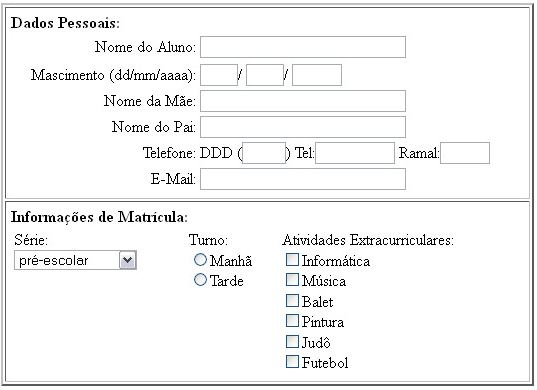
\includegraphics[width=\linewidth]{img/formulario.png}

    \label{fig:enter-label}
\end{figure}
    
\end{frame}



\begin{frame}
  \frametitle{Novos Elementos em Formulários HTML5}

  O HTML5 introduziu vários novos elementos para melhorar a semântica e funcionalidade dos formulários.

  \begin{itemize}
    \item \texttt{<input type="email"}\texttt{>} - Campo de Email
    \item \texttt{<input type="url"}\texttt{>} - Campo de URL
    \item \texttt{<input type="tel"}\texttt{>} - Campo de Telefone
    \item \texttt{<input type="number"}\texttt{>} - Campo Numérico
    \item \texttt{<input type="date"}\texttt{>} - Campo de Data
    \item \texttt{<input type="color"}\texttt{>} - Seletor de Cor
    \item \texttt{<input type="range"}\texttt{>} - Controle de Intervalo
    \item \texttt{<datalist>} - Lista de Dados para Campos de Texto
    \item \texttt{<textarea>} - Área de Texto Multilinhas
    \item \texttt{<output>} - Resultado ou Cálculo de Formulário
  \end{itemize}
\end{frame}

\begin{frame}[fragile]
  \frametitle{Campo de Email em HTML5 (\texttt{<input type="email"}\texttt{>})}

  O elemento \texttt{<input type="email"}\texttt{>} é usado para campos de entrada de endereço de email. Atributos importantes:

  \begin{itemize}
    \item \texttt{name} - Nome do campo.
    \item \texttt{id} - Identificador único do campo.
    \item \texttt{required} - Indica que o campo é obrigatório.
    \item \texttt{placeholder} - Texto de exemplo exibido no campo.
    \item \texttt{pattern} - Define uma expressão regular para validar o formato do email.
  \end{itemize}

\begin{block}{Exemplo}
  \begin{verbatim}
  <label for="email">Endereço de Email:</label>
  <input type="email" id="email" name="email" required
         placeholder="seuemail@example.com"
         pattern="[a-z0-9._%+-]+@[a-z0-9.-]+\.[a-z]{2,4}$">
  \end{verbatim}
\end{block}
\end{frame}

\begin{frame}[fragile]
  \frametitle{Campo de URL em HTML5 (\texttt{<input type="url"}\texttt{>})}

  O elemento \texttt{<input type="url"}\texttt{>} é usado para campos de entrada de URLs. Atributos importantes:

  \begin{itemize}
    \item \texttt{name} - Nome do campo.
    \item \texttt{id} - Identificador único do campo.
    \item \texttt{required} - Indica que o campo é obrigatório.
    \item \texttt{placeholder} - Texto de exemplo exibido no campo.
    \item \texttt{multiple} - Mais de uma entrada, seguida de (,).
    \item \texttt{pattern} - Define uma expressão regular para validar a URL.
  \end{itemize}
  
\begin{block}{Exemplo}
  \begin{verbatim}
  <label for="website">Website:</label>
  <input type="url" id="website" name="website" required
         placeholder="https://www.example.com"
         pattern="https?://.*">
  \end{verbatim}    
\end{block}

\end{frame}


\begin{frame}[fragile]
  \frametitle{Campo de Telefone em HTML5 (\texttt{<input type="tel"}\texttt{>})}

  O elemento \texttt{<input type="tel"\texttt{>}} é usado para campos de entrada de números de telefone. Atributos importantes:
  \begin{itemize}
    \item \texttt{name} - Nome do campo.
    \item \texttt{id} - Identificador único do campo.
    \item \texttt{required} - Indica que o campo é obrigatório.
    \item \texttt{placeholder} - Texto de exemplo exibido no campo.
    \item \texttt{pattern} - Define uma expressão regular para validar o formato do telefone.
  \end{itemize}

  \begin{block}{Exemplo}
    \begin{verbatim}
    <label for="phone">Telefone:</label>
    <input type="tel" id="phone" name="phone" required
           placeholder="(XX) XXXX-XXXX"
           pattern="\(\d{2}\) \d{4}-\d{4}">
    \end{verbatim}
  \end{block}
\end{frame}



\begin{frame}[fragile]
  \frametitle{Campo Numérico em HTML5 (\texttt{<input type="number"}\texttt{>})}

  O elemento \texttt{<input type="number"}\texttt{>} é usado para campos de entrada numérica.  Atributos importantes:

  \begin{itemize}
    \item \texttt{name} - Nome do campo.
    \item \texttt{id} - Identificador único do campo.
    \item \texttt{min} e \texttt{max} - Definem o intervalo mínimo e máximo de valores.
    \item \texttt{step} - Define o incremento para aumentar ou diminuir o valor.
    \item \texttt{value} - Define o valor inicial.
    \item \texttt{required} - Indica que o campo é obrigatório.
  \end{itemize}

  \begin{block}{Exemplo}
    \begin{verbatim}
    <label for="quant">Quantidade:</label>
    <input type="number" id="quantity" name="quant"
           min="1" max="10" step="1" value="1" required>
    \end{verbatim}
  \end{block}
\end{frame}


\begin{frame}[fragile]
  \frametitle{Campo de Data em HTML5 (\texttt{<input type="date"...>})}

  O elemento \texttt{<input type="date" ...>} é usado para campos de entrada de datas. Atributos importantes:

  \begin{itemize}
    \item \texttt{name} - Nome do campo.
    \item \texttt{id} - Identificador único do campo.
    \item \texttt{min} e \texttt{max} - Definem o intervalo mínimo e máximo de datas.
    \item \texttt{value} - Define o valor inicial.
    \item \texttt{required} - Indica que o campo é obrigatório.
  \end{itemize}

  \begin{block}{Exemplo}
    \begin{verbatim}
    <label for="dob">Data de Nascimento:</label>
    <input type="date" id="dob" name="dob"
           min="1900-01-01" max="2023-12-31" required>
    \end{verbatim}
  \end{block}
\end{frame}


\begin{frame}[fragile]
  \frametitle{Seletor de Cor em HTML5 (\texttt{<input type="color" ...>})}

  O elemento \texttt{<input type="color" ...>} é usado para campos de seleção de cor. Atributos importantes:

  \begin{itemize}
    \item \texttt{name} - Nome do campo.
    \item \texttt{id} - Identificador único do campo.
    \item \texttt{value} - Define a cor inicial selecionada (formato hexadecimal).
    \item \texttt{required} - Indica que o campo é obrigatório.
  \end{itemize}

  \begin{block}{Exemplo}
    \begin{verbatim}
    <label for="color">Escolha uma cor:</label>
    <input type="color" id="color" name="color"
           value="#ff0000" required>
    \end{verbatim}
  \end{block}
\end{frame}


\begin{frame}[fragile]
  \frametitle{Intervalo em HTML5 (\texttt{<input type="range" ...>})}

  O elemento \texttt{<input type="range" ...>} é usado para criar controles de intervalo (faixas deslizantes). Atributos importantes:

  \begin{itemize}
    \item \texttt{min} e \texttt{max} - Definem o intervalo mínimo e máximo de valores.
    \item \texttt{step} - Define o incremento para ajustar o valor.
    \item \texttt{value} - Define o valor inicial.
  \end{itemize}

  \begin{block}{Exemplo}
    \begin{verbatim}
    <label for="volume">Volume:</label>
    <input type="range" id="volume" name="volume"
           min="0" max="100" step="1" value="50">
    \end{verbatim}
  \end{block}
\end{frame}


\begin{frame}[fragile]
  \frametitle{Intervalo com Ticks (\texttt{<input type="range" ...>})}

  O elemento \texttt{<input type="range" ...>} pode incluir marcas de seleção (ticks) para indicar valores específicos.

  \begin{block}{Exemplo com Ticks}
    \begin{verbatim}
    <label for="brightness">Brilho:</label>
    <input type="range" id="brightness" name="brightness"
           min="0" max="100" step="10" value="50"
           list="tickmarks">
    <datalist id="tickmarks">
      <option value="0">
      <option value="25">
      <option value="50">
      <option value="75">
      <option value="100">
    </datalist>
    \end{verbatim}
  \end{block}
\end{frame}


\begin{frame}[fragile]
  \frametitle{Elemento \texttt{<datalist>} em HTML5}

  O elemento \texttt{<datalist>} é usado para fornecer uma lista de opções predefinidas para um campo de entrada.

  \begin{block}{Exemplo com \texttt{<datalist>}}
    \begin{verbatim}
    <label for="browser">Navegador:</label>
    <input type="text" id="browser" name="browser" 
    list="browsers">
    <datalist id="browsers">
      <option value="Chrome">
      <option value="Firefox">
      <option value="Edge">
      <option value="Safari">
      <option value="Opera">
    </datalist>
    \end{verbatim}
  \end{block}
\end{frame}


\begin{frame}[fragile]
  \frametitle{Campo de Texto Multilinha em HTML5 (\texttt{<textarea>})}

  O elemento \texttt{<textarea>} é usado para campos de texto multilinha. Atributos importantes:

  \begin{itemize}
    \item \texttt{rows} e \texttt{cols} - Número de linhas e colunas do campo.
    \item \texttt{placeholder} - Texto de exemplo exibido no campo.
    \item \texttt{required} - Indica que o campo é obrigatório.
    \item \texttt{maxlength} - Número máximo de caracteres permitidos.
  \end{itemize}

  \begin{block}{Exemplo com \texttt{<textarea>}}
    \begin{verbatim}
    <label for="comments">Comentários:</label>
    <textarea id="comments" name="comments"
              rows="4" cols="40"
              placeholder="Digite seus comentários..."
              required maxlength="200"></textarea>
    \end{verbatim}
  \end{block}
\end{frame}


\begin{frame}[fragile]
  \frametitle{Elemento \texttt{<output>} em HTML5}

  O elemento \texttt{<output>} é usado para exibir o resultado de um cálculo ou processamento. 

  \begin{block}{Exemplo com \texttt{<output>}}
    \begin{verbatim}
    <form oninput="result.value=parseInt(a.value) + 
        parseInt(b.value)">
      <label for="a">Número A:</label>
      <input type="number" id="a" name="a" value="0">
      +
      <label for="b">Número B:</label>
      <input type="number" id="b" name="b" value="0">
      =
      <output name="result">0</output>
    </form>
    \end{verbatim}
  \end{block}
\end{frame}

\begin{frame}[fragile]
  \frametitle{Elementos \texttt{<fieldset>} e \texttt{<legend>}}

  Os elementos \texttt{<fieldset>} e \texttt{<legend>} são usados para agrupar e identificar elementos relacionados de um formulário.

  \begin{block}{Exemplo com \texttt{<fieldset>} e \texttt{<legend>}}
    \begin{verbatim}
    <form>
      <fieldset>
        <legend>Informações Pessoais</legend>
        <label for="name">Nome:</label>
        <input type="text" id="name" name="name">
        <br>
        <label for="email">E-mail:</label>
        <input type="email" id="email" name="email">
      </fieldset>
    </form>
    \end{verbatim}
  \end{block}
\end{frame}


\begin{frame}
\frametitle{Elementos \texttt{<fieldset>} e \texttt{<legend>}}
\begin{figure}
    \centering
    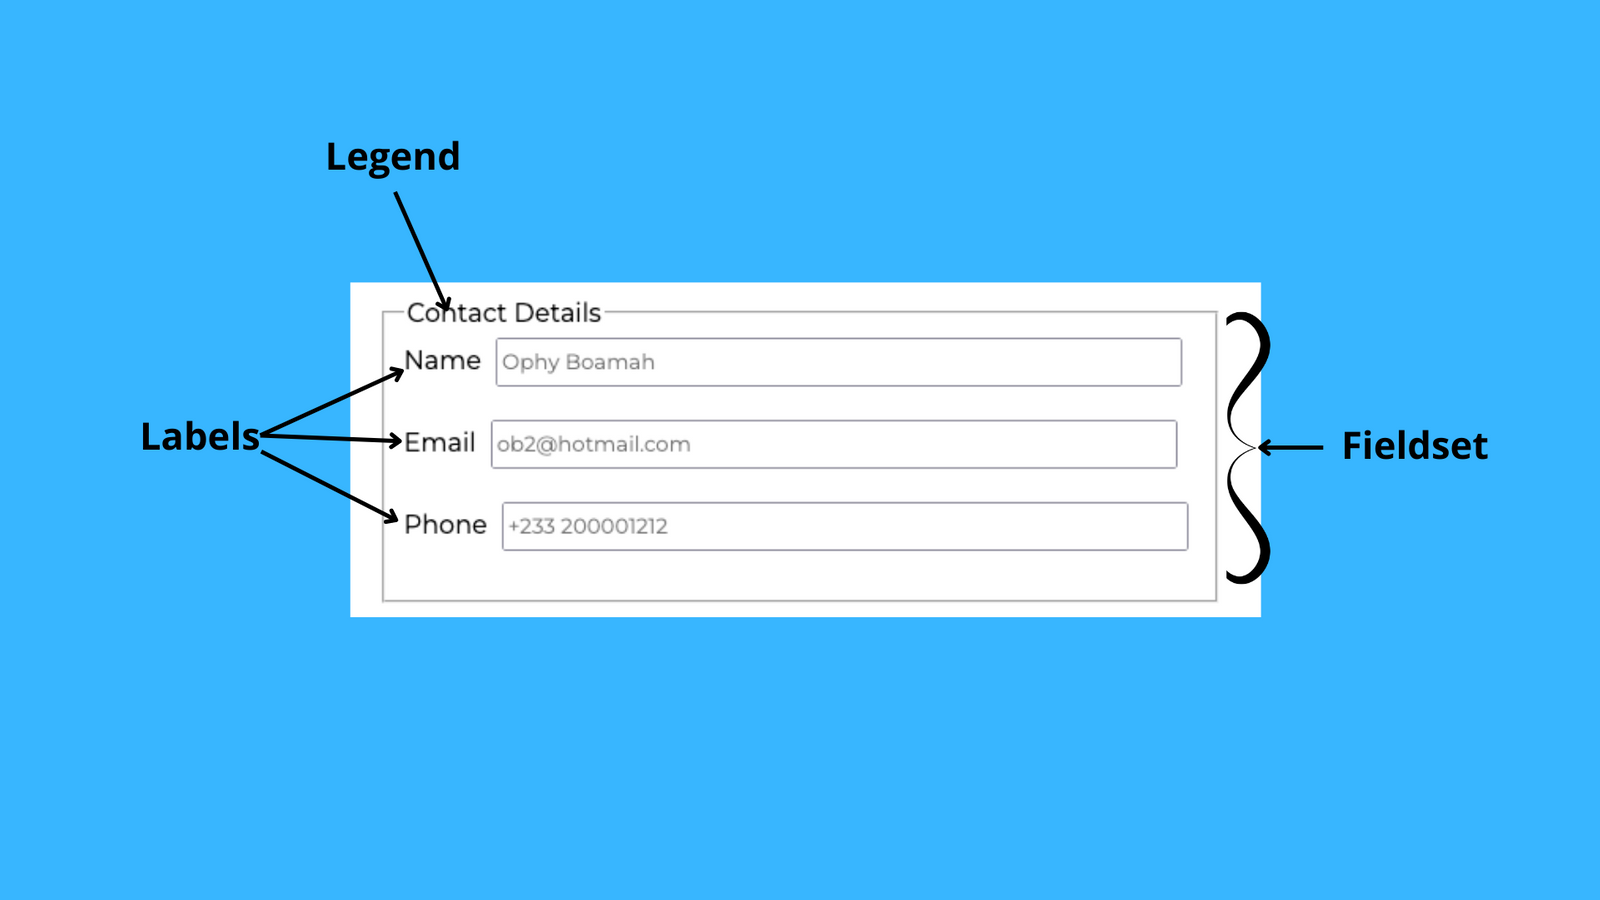
\includegraphics[width=\linewidth]{img/Fieldset-2.png}

\end{figure}

\end{frame}


\begin{frame}[fragile]
  \frametitle{Elemento \texttt{<map>} em HTML}

  O elemento \texttt{<map>} é usado em conjunto com a tag \texttt{<area>} para criar mapas de imagem sensíveis a cliques em HTML.

  \begin{block}{Uso do \texttt{<map>}}
    \begin{verbatim}
<img src="mapa.png" usemap="#imagemMapa">
<map name="imagemMapa">
  <area shape="rect" coords="0,0,100,100" href="link1.html"
    alt="Área 1">
  <area shape="circle" coords="150,150,50" href="link2.html"
    alt="Área 2">
  <area shape="poly" coords="200,50,250,100,200,150" 
    href="link3.html" alt="Área 3">
</map>
    \end{verbatim}
  \end{block}

  As áreas especificadas pelas tags \texttt{<area>} definem regiões clicáveis na imagem, redirecionando o usuário para diferentes páginas ou ações.

\end{frame}

\begin{frame}[fragile]
  \frametitle{Formas para Áreas de Mapa Sensíveis em HTML}

  O atributo \texttt{shape} da tag \texttt{<area>} é usado para definir a forma da área clicável em um mapa de imagem.

  \begin{block}{Valores para o atributo \texttt{shape}}
    \begin{itemize}
      \item \texttt{rect} - Retângulo
      \item \texttt{circle} - Círculo
      \item \texttt{poly} - Polígono
      \item \texttt{default} - Área padrão (quando não há correspondência com outras áreas)
    \end{itemize}
  \end{block}


\end{frame}


\begin{frame}
  \frametitle{Elemento \texttt{<map>} em HTML}

Formatos aceitos.

  \begin{center}
    \begin{tikzpicture}
      % Retângulo
      \draw[blue, thick] (0, 0) rectangle (3, 2);
      \node[blue] at (1.5, 1) {Retângulo};

      % Círculo
      \draw[red, thick] (5, 1) circle (1);
      \node[red] at (5, 0.5) {Círculo};

      % Polígono
      \draw[green, thick] (9, 0) -- (10.5, 0) -- (11, 1) -- (10, 2) -- cycle;
      \node[green] at (10.5, 1) {Polígono};
    \end{tikzpicture}
  \end{center}
\end{frame}



\begin{frame}{Elemento \texttt{<map>} em HTML}

Como pegar os poligonos

\begin{figure}
    \centering
    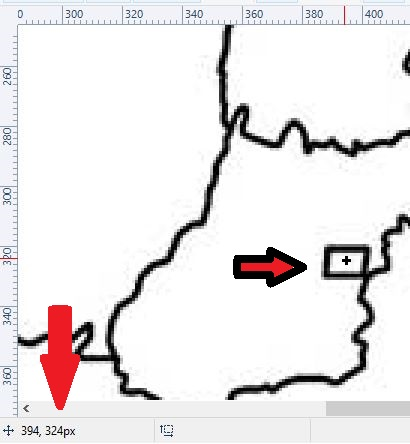
\includegraphics[width=0.4\linewidth]{img/paint-map.JPG}
    \caption{MS Paint}
    \label{fig:enter-label}
\end{figure}

\textbf{Dica:} Ferramentas como \href{http://www.image-map.net/}{http://www.image-map.net/} podem ajudar a pegar coordenadas precisas para as áreas.

  \begin{itemize}
    \item Evita cálculos manuais e erros.
    \item Facilita a criação de mapas complexos.
  \end{itemize}

\end{frame}


\begin{frame}[fragile]
  \frametitle{Elemento \texttt{<iframe>} em HTML}

  O elemento \texttt{<iframe>} é usado para incorporar conteúdo de outros documentos HTML em uma página.

  \begin{itemize}
    \item Permite exibir uma página da web dentro de outra página.
    \item Pode exibir conteúdo de outro domínio.
    \item Usado para incorporar mapas, vídeos, widgets, etc.
  \end{itemize}

  \vspace{1em}

\begin{block}{Exemplo}
\begin{verbatim}
<iframe src="https://example.com" width="500" height="300">
</iframe>
\end{verbatim}    
\end{block}
  
\end{frame}

\begin{frame}[fragile]
  \frametitle{Elemento \texttt{<iframe>} em HTML}

  O elemento \texttt{<iframe>} especifica um quadro incorporado (inline frame).

  \begin{itemize}
    \item O atributo \texttt{src} define a URL da página a ser incorporada.
    \item Sempre inclua o atributo \texttt{title} (para leitores de tela).
    \item Os atributos \texttt{height} e \texttt{width} especificam o tamanho do iframe.
    \item Use \texttt{border:none;} para remover a borda ao redor do iframe.
  \end{itemize}

  \vspace{1em}

\begin{block}{Exemplo}
\begin{verbatim}
<iframe src="https://www.ifspcjo.edu.br" width="500" 
height="300" title="Exemplo"></iframe>
\end{verbatim}    
\end{block}
  
\end{frame}


\begin{frame}{Exercício \texttt{iframe}}

Criar um iframe: 
\begin{itemize}
    \item Mapa do google maps;
    \item Vídeo do youtube.
\end{itemize}
    
\end{frame}


\end{document}
